\documentclass{article}
\usepackage[margin=1in]{geometry}
\usepackage{amsmath,amsthm,amssymb}
\usepackage{bbm,enumerate,mathtools}
\usepackage{tikz,pgfplots}
\usepackage{chessboard}
\usepackage[hidelinks]{hyperref}
\usepackage{multicol} % Problem 35

\newenvironment{question}{\begin{trivlist}\item[\textbf{Question.}]}{\end{trivlist}}
\newenvironment{note}{\begin{trivlist}\item[\textbf{Note.}]}{\end{trivlist}}
\newenvironment{references}{\begin{trivlist}\item[\textbf{References.}]}{\end{trivlist}}
\newenvironment{related}{\begin{trivlist}\item[\textbf{Related.}]\end{trivlist}\begin{enumerate}}{\end{enumerate}}


\begin{document}
\rating{3}{3}
One way to form minimum perimeter polyominoes is to arrange the tiles in a
square spiral, however, there are often minimal-perimeter configurations that
are not formed by a square spiral.
\begin{figure}[ht!]
  \centering
  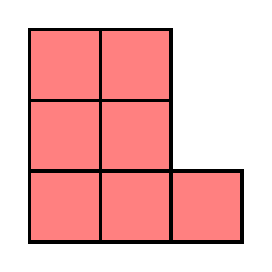
\begin{tikzpicture}[scale=0.9]
    \foreach \x/\y in {
      0/2, 1/2,
      0/1, 1/1,
      0/0, 1/0, 2/0} {
      \draw[very thick, fill={red!50}] (\x,\y) rectangle (\x+1,\y+1);
    }
  \end{tikzpicture}
  ~~~
  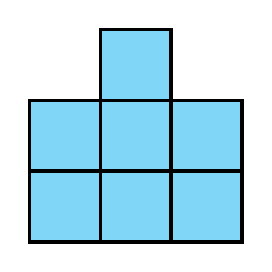
\begin{tikzpicture}[scale=0.9]
    \foreach \x/\y in {
           1/2,
      0/1, 1/1, 2/1,
      0/0, 1/0, 2/0} {
      \draw[very thick, fill={cyan!50}] (\x,\y) rectangle (\x+1,\y+1);
    }
  \end{tikzpicture}
  ~~~
  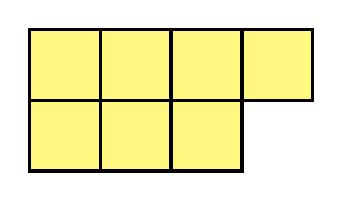
\begin{tikzpicture}[scale=0.9]
    \foreach \x/\y in {
      0/1, 1/1, 2/1, 3/1,
      0/0, 1/0, 2/0} {
      \draw[very thick, fill={yellow!50}] (\x,\y) rectangle (\x+1,\y+1);
    }
  \end{tikzpicture}
  ~~~
  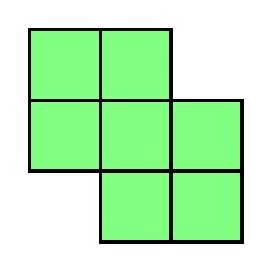
\begin{tikzpicture}[scale=0.9]
    \foreach \x/\y in {
      0/2, 1/2,
      0/1, 1/1, 2/1,
           1/0, 2/0} {
      \draw[very thick, fill={green!50}] (\x,\y) rectangle (\x+1,\y+1);
    }
  \end{tikzpicture}
  \caption{
    All $\operatorname{A100092}(7) = 4$ minimal-perimeter $7$-ominoes, the first
    of which is the beginning of a square spiral.
  }
\end{figure}
\begin{question}
  Given (pseudo-)polyforms on some plane tiling, what is the minimum perimeter
  of a region containing $n$ cells?
\end{question}

\begin{note}
  In the case of the pseudo-polyform on a snub square tiling, a spiral does not
  appear to be the way to minimize the perimeter of an $n$-form.
\end{note}

\begin{related}
  \item How many such minimal-perimeter regions exist? How many regions have
  some sort of symmetry?
  \item What is the minimum perimeter if the region must be symmetric under
  mirror image? Under $180^\circ$ rotation?
  \item What do these look like on the ``ordinary'' polyforms:
  polyominoes, polyiamonds, polyhexes, etc.
  \item Next, what about the pseudo-polyforms that specifically live on the
  snub square tiling, truncated hexagonal tiling, and all of the fifteen
  pentagonal tilings?
  \item What about irregular tilings like the Penrose tiling?
  \item What about higher dimenional tilings, and minimizing side lengths or
  surface area or both?
  \item What about (pseudo-)polyforms that can't cover the plane or don't
  correspond to a tiling (e.g. polypents)
  \item What about minimizing (or maximizing) via other metrics?
  The perimeter of the convex hull? The sum of the angles? The number of
  sides touching internally?
  \item What is the minimum perimeter region that can contain all free
  (pseudo-)$n$-forms? Fixed forms?
  How many fillings does minimal-perimeter region have?
\end{related}
\begin{references}
  \item Problems 72 and 77.
  \item \url{https://oeis.org/A027709}
  \item \url{https://oeis.org/A100092}
\end{references}
\end{document}
